\documentclass[conference]{IEEEtran}
\IEEEoverridecommandlockouts
\usepackage{matlab-prettifier}
\usepackage{cite}
\usepackage{amsmath,amssymb,amsfonts}
\usepackage{nccmath}
\usepackage{algorithmic}
\usepackage{graphicx}
\usepackage{textcomp}
\usepackage{xcolor}
\usepackage{float}
\usepackage{tabularx}
\def\BibTeX{{\rm B\kern-.05em{\sc i\kern-.025em b}\kern-.08em
    T\kern-.1667em\lower.7ex\hbox{E}\kern-.125emX}}

\begin{document}

\title{Project 2 : Range Doppler Matrix Generation for an LFM Radar System}

\author{\IEEEauthorblockN{Owen Sowatzke}
\IEEEauthorblockA{\textit{Electrical Engineering Department} \\
\textit{University of Arizona}\\
Tucson, USA \\
osowatzke@arizona.edu}}
\maketitle

\begin{abstract}
The range resolution of a radar system is inversely proportional to the bandwidth of its transmitted waveform. To achieve a fine range resolution, a high bandwidth waveform is required. This typically results in an increased ADC sampling rate, which leads to higher production costs. A linear frequency modulated (LFM) waveform can be used in conjunction with stretch processing to provide a large transmitted waveform bandwidth with a reduced ADC sampling rate. This provides a fine range resolution at reduced production costs. This document provides an overview of an LFM radar system with a focus on the signal processing. It specifically examines the generation of range doppler matrices (RDMs) using range and doppler compression. The effects of amplitude compensation, range windowing, and doppler windowing are also be examined. Finally, the measurement limitations of the LFM radar system are examined and methods for improving these limitations are discussed. 
\end{abstract}

\begin{IEEEkeywords}
Linear Frequency Modulated (LFM) Radar System, Stretch Processing, Range Doppler Matrix, Range Compression, Doppler Compression, Amplitude Compensation, Range Windowing, Doppler Windowing, Range Resolution, Velocity Resolution, Range Ambiguity, Velocity Ambiguity
%Pulse Compression, Linear Frequency Modulated (LFM) Waveform, Matched Filter, SNR, Range Resolution
\end{IEEEkeywords}
\section{Introduction}
In this document, an LFM radar system that leverages stretch processing will be examined. The radar system of interest with configured with the following parameters:
\begin{table}[H]
\caption{Radar System Parameters}
\label{Parameter Table}
\begin{tabularx}{0.5\textwidth}{| X | X |}
\hline
Carrier Frequency & 77 GHz \\
\hline
Sweep Frequency & 76.8 GHz - 77.2 GHz \\
\hline
Pulse Width & 20 $\mu s$ \\
\hline
PRI & 30 $\mu s$ \\
\hline
Fast Time Samples & 400 \\
\hline 
Number of Chirps & 500 \\
\hline
Fast Time Sampling Frequency & 20 MHz \\
\hline
\end{tabularx}
\end{table}
\noindent
The system's ADC data will be generated for a variety of scenarios using MATLAB. Then, signal processing will be performed on this data to generate Range Doppler Matrices (RDMs).
\par
This document will provide a walk-through of the data generation and signal processing with simulation results that highlight key milestones. These milestones include ADC data generation, range and doppler compression, amplitude compensation, and range and doppler windowing. Finally, the measurement limitations of the system will be examined, and methods for improving these limitations will be discussed.
\section{ADC Data Generation}
The target returns for a radar system are delayed and doppler shifted versions of the transmitted signal. For an LFM radar system, the transmitted signal takes the following form:
\begin{equation}
x(t) = e^{j\pi\beta t^2/\tau}
\end{equation}
The instantaneous frequency of this signal is given by the following equation:
\begin{equation}
F_i(t) = \frac{1}{2\pi}\frac{d\theta(t)}{dt} = \frac{\beta}{\tau}t
\end{equation}
If the instantaneous frequency of the transmitted waveform is plotted versus time, the result will be a ramp function. For a target at a constant range (static target), the received signal will be a delayed ramp function. If target velocity is added, a DC offset will be added to the delayed ramp function. This is illustrated in Fig. \ref{instantaneous_frequency}.
\begin{figure}[H]
\centerline{\fbox{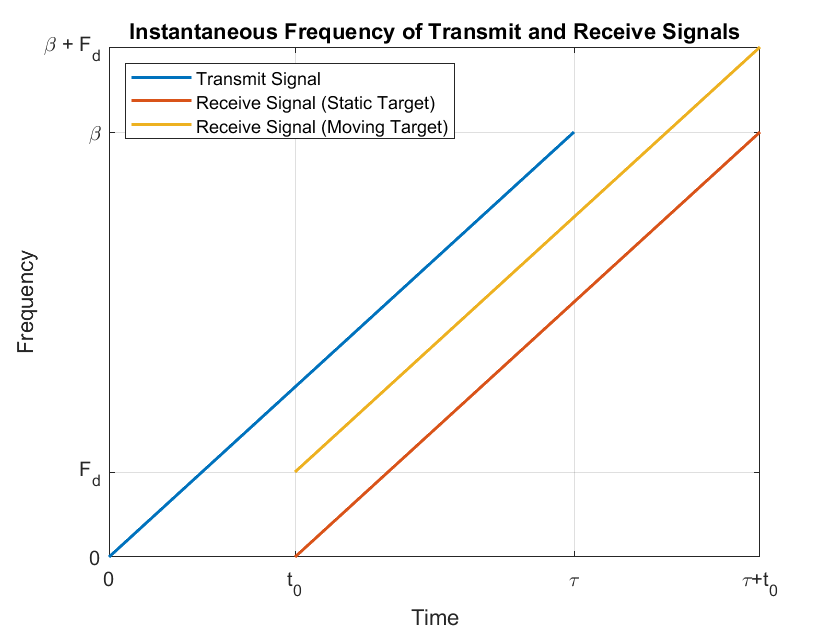
\includegraphics[width=0.4\textwidth]{instantaneous_frequency.png}}}
\caption{Instantaneous Frequency of Transmit and Receive Signals.}
\label{instantaneous_frequency}
\end{figure}
If the targets returns are sampled directly, a sample rate of at least $\beta$ is required. In the stretch processing receiver, additional analog processing is performed prior to sampling to reduce the sample rate and to simplify the signal processing. This analog processing involves mixing the received signal with an inverted chirp of the following form:
\begin{equation}
m(t) = e^{-j\pi\beta t^2/\tau}
\end{equation}
After mixing, the beat frequency of each target return is constant with respect to time as shown in Fig. \ref{beat_frequency}.
\begin{figure}[H]
\centerline{\fbox{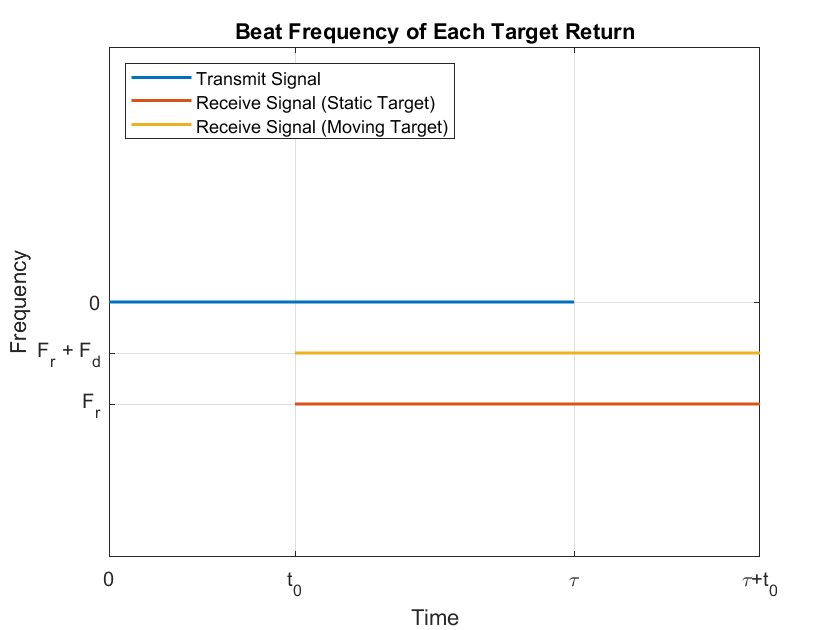
\includegraphics[width=0.4\textwidth]{beat_frequency.png}}}
\caption{Beat Frequency of Each Target Return}
\label{beat_frequency}
\end{figure}
Note that the beat frequencies start and stop at different times. This phenomenon is called range skew. An analog filter can be used to compensate for the range skew. Since the doppler shift of the target is small with respect to the range frequency, the time delay of each beat frequency can be approximated as follows:
\begin{equation}
t_d \approx -\frac{\tau(F_r+F_d)}{\beta} = -\frac{\tau F_b}{\beta}
\end{equation}
Therefore, the analog filter should provide a group delay of $\frac{\tau F_b}{\beta}$ seconds at a frequency of $F_b$ Hz. The group delay of an analog filter can be expressed in terms of the phase of the frequency response as follows:
\begin{equation}
d_g(\Omega) = -\frac{d\Phi(\Omega)}{d\Omega}
\end{equation}
Therefore, the frequency response of the delay compensation filter should have the following phase:
\begin{equation}
\Phi(\Omega) = -\int d_g(\Omega)d\Omega = -\int\frac{\tau\Omega}{2\pi\beta}d\Omega = -\frac{\tau\Omega^2}{4\pi\beta}
\end{equation}
Note that the amplitude of the frequency response should be constant to prevent distortion of targets returns at different ranges (different frequencies). Therefore, the frequency response of the desired analog filter is given by the following equation:
\begin{equation}
H(\Omega) = e^{-j\tau\Omega^2/(4\pi\beta)}
\end{equation} 
After the analog filter is applied, the time-frequency plot in Fig. \ref{beat_frequency_analog_filter} results.
\begin{figure}[H]
\centerline{\fbox{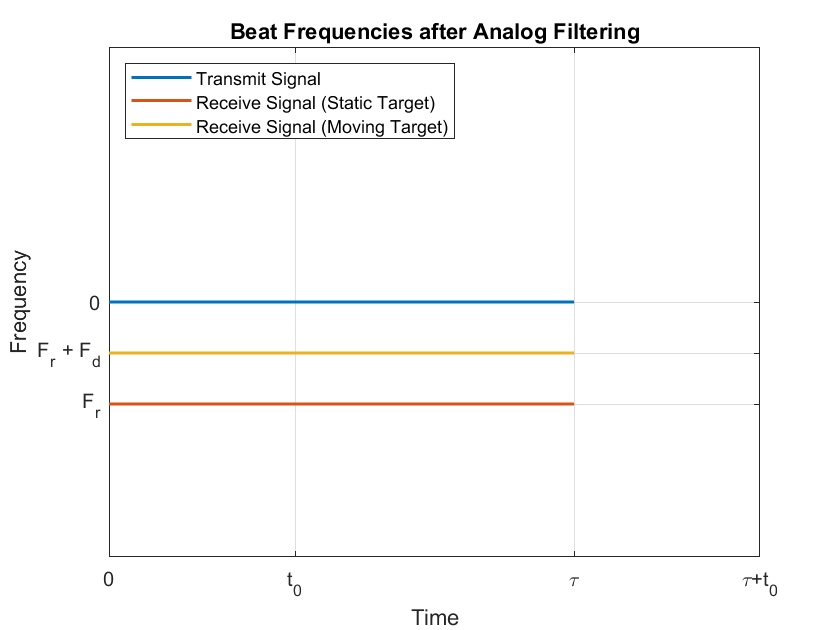
\includegraphics[width=0.4\textwidth]{beat_frequency_analog_filter.png}}}
\caption{Beat Frequencies after Analog Filtering}
\label{beat_frequency_analog_filter}
\end{figure}
For a properly-designed radar system, the range gate size should be large enough to prevent target motion across range gates during the CPI. If this is the case, the stop-and-hop approximation can be used. This approximation decomposes each target return into two parts. The first part of the target return occurs due to the target's range and repeats each PRI. The second part of the target returns occurs due to the doppler shift, which is applied across the entire train of pulses. Using this approximation, the received data cube can be generated in MATLAB as follows:
\begin{figure}[H]
\centerline{\fbox{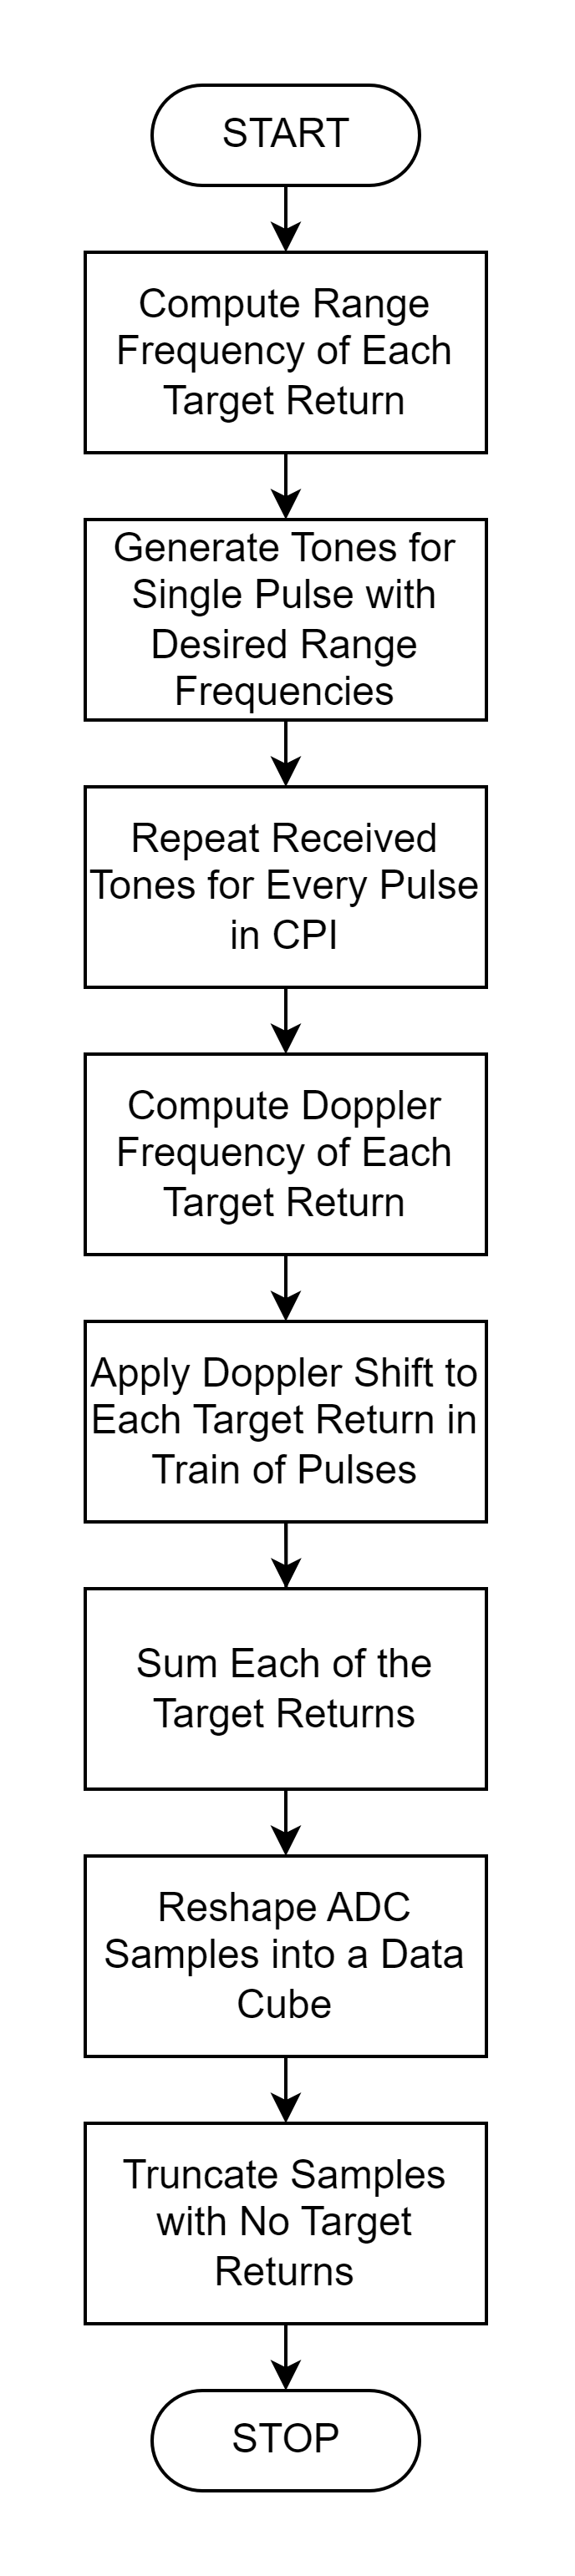
\includegraphics[width=0.14\textwidth]{adc_signal_generation_bd.png}}}
\caption{Received Data Cube Generation.}
\label{adc_signal_generation_bd}
\end{figure}
\section{Range and Doppler Compression}
An RDM can be generated from the received data cube using range and doppler compression. This is done by taking an FFT along the fast-time axis and another FFT along the slow-time axis.
\begin{figure}[H]
\centerline{\fbox{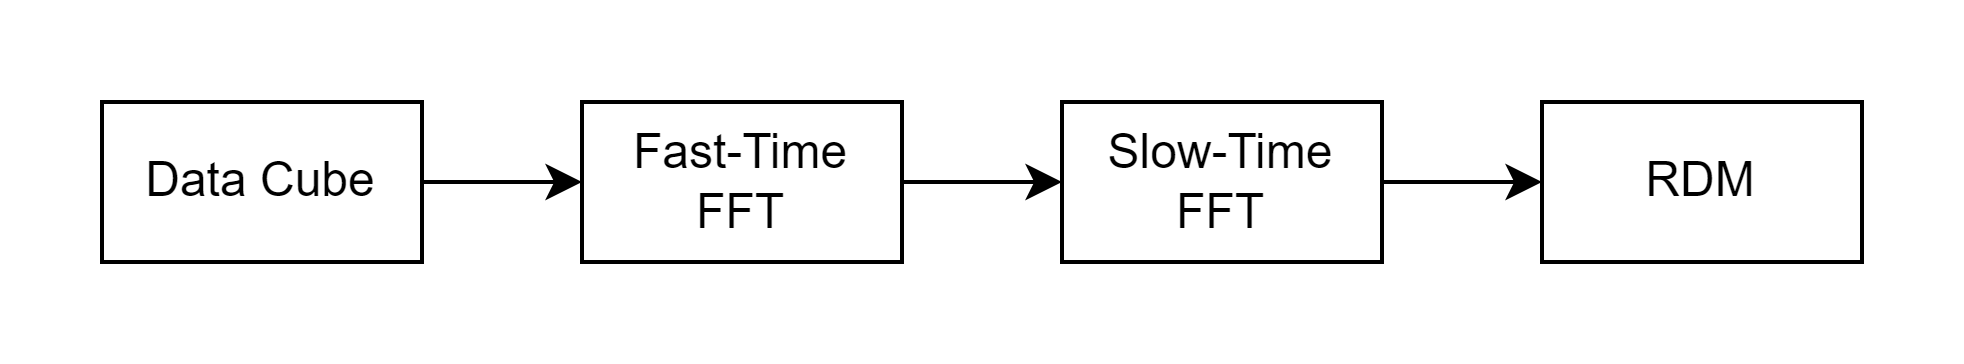
\includegraphics[width=0.4\textwidth]{range_doppler_compression_bd.png}}}
\caption{Range and Doppler Compression.}
\label{range_doppler_compression_bd}
\end{figure}
\noindent
The fast-time FFT extracts the frequency content in each pulse. Each pulse contains the sum of target returns (tones). Therefore, the fast-time FFT will produce a peak for each target. The frequency of each peak is influenced primarily by target range. As such, it is used to measure range; however, the doppler shift of the target will produce the following error in range measurements:
\begin{equation}
\delta R = -\frac{c\tau F_d}{2\beta}
\end{equation}
The slow-time FFT measures doppler shift or velocity of the target. The slow-time FFT is not be influenced by the range of the target.
\par
Because the radar system is using an upchirp, the target's range frequency ($F_r$) will be given by the following: 
\begin{equation}
F_r = -\frac{\beta t_d}{\tau} = -\frac{2\beta R}{c\tau}
\end{equation}
Note that targets at non-zero ranges will result in negative beat frequencies. This results in the small ranges being wrapped to the top of the RDM as illustrated in Fig. \ref{unsorted_rdm}.
\begin{figure}[H]
\centerline{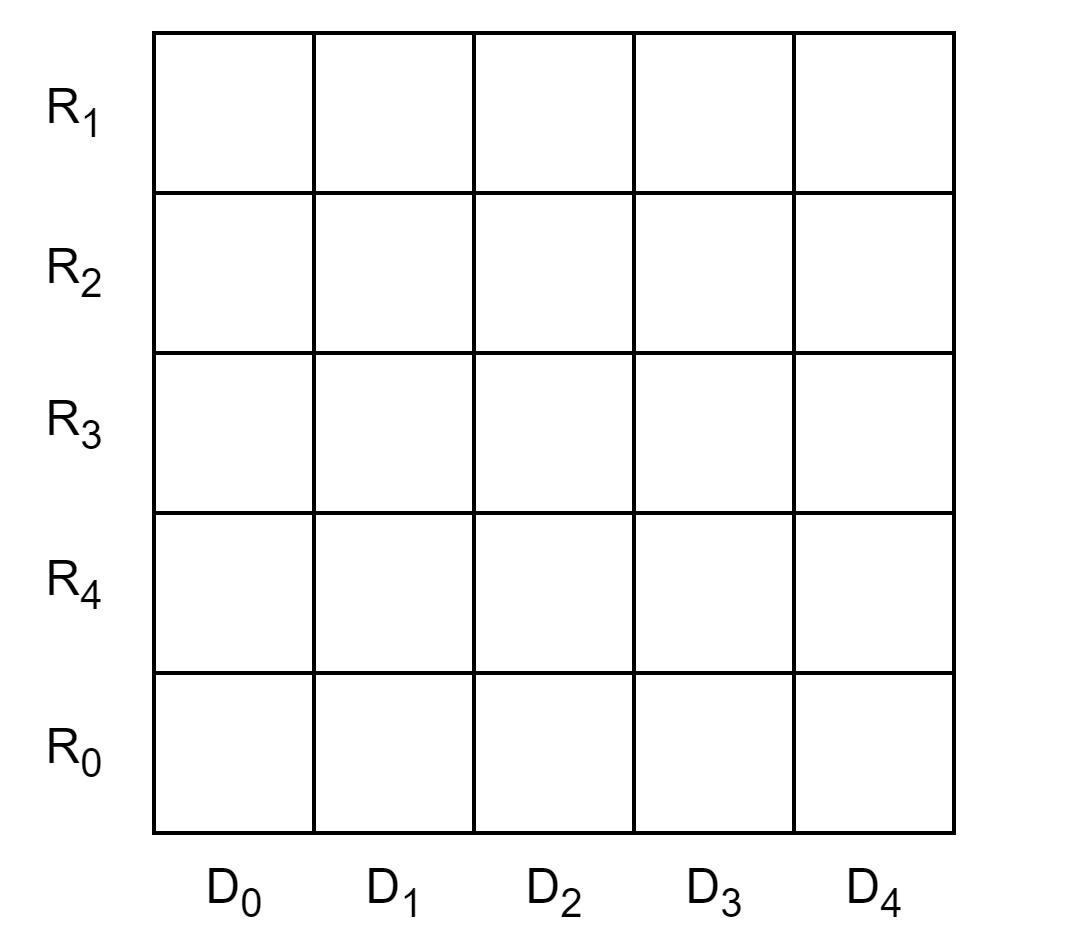
\includegraphics[width=0.3\textwidth]{unsorted_rdm.png}}
\caption{Unsorted RDM.}
\label{unsorted_rdm}
\end{figure}
\noindent
The range bins can be sorted in ascending order by flipping the RDM along the fast-time axis and circular shifting range bin zero to the bottom of the RDM. After this manipulation, the RDM in Fig. \ref{sorted_rdm} results.
\begin{figure}[H]
\centerline{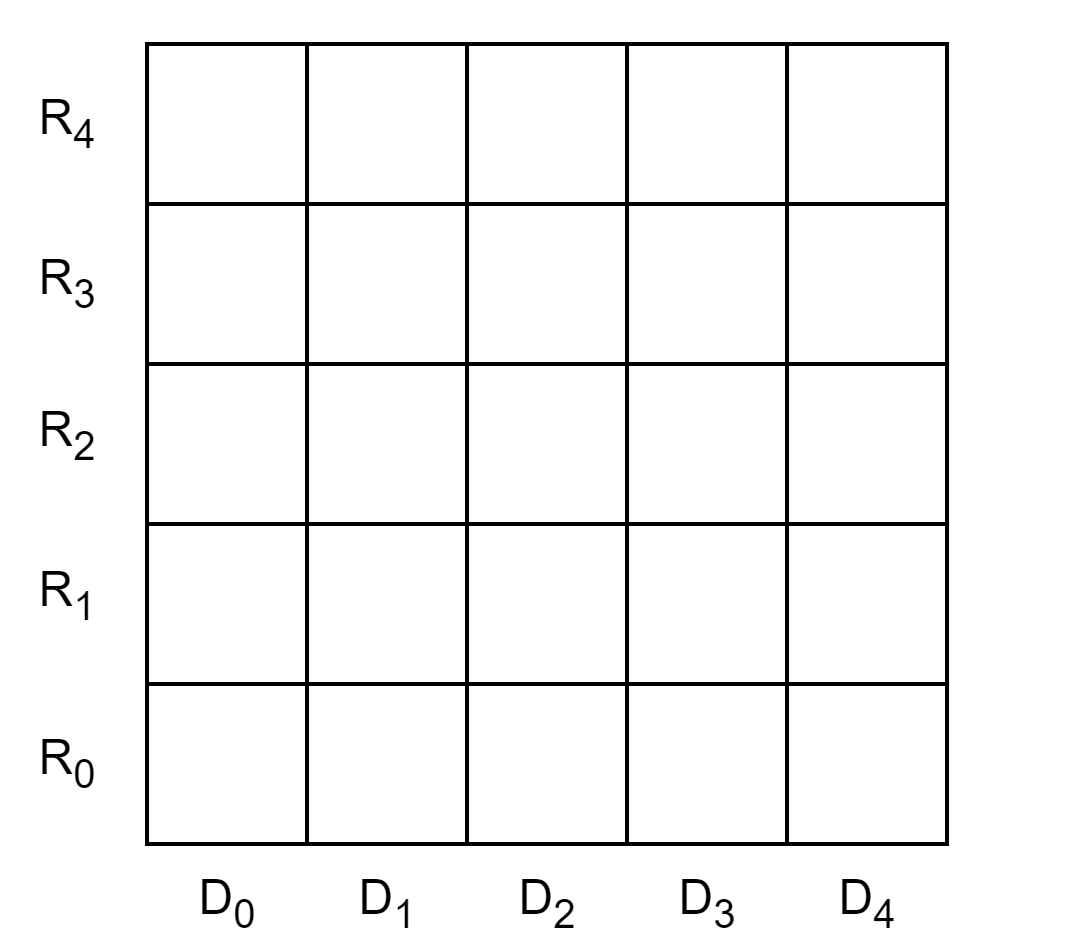
\includegraphics[width=0.3\textwidth]{sorted_rdm.png}}
\caption{Sorted RDM.}
\label{sorted_rdm}
\end{figure}
\noindent
Note that this sorting operation is typically performed in post-processing. However, in this document, it will be performed earlier to simplify the amplitude compensation applied before the slow-time FFT. After the range gate reordering, the RDM can be generated according to the following block diagram:
\begin{figure}[H]
\centerline{\fbox{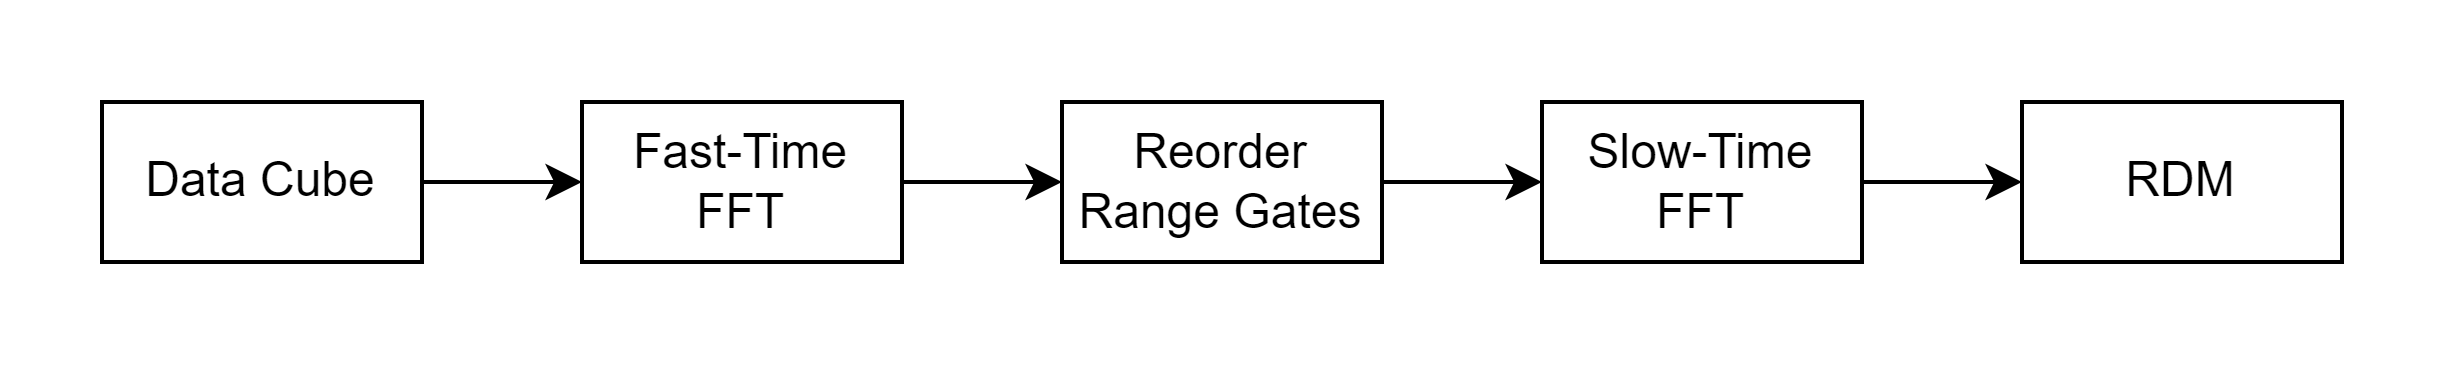
\includegraphics[width=0.4\textwidth]{gate_reordering_bd.png}}}
\caption{RDM Generation with Gate Reordering}
\label{gate_reordering_bd}
\end{figure}
\par
Consider the return from two targets without thermal noise. Let the first target be located at a range of $10m$ with a velocity of $15m/s$ and an RCS of $1m^2$. Next, let the second target be located at a range of $100m$ with a velocity of $10m/s$ and an RCS of $10000m^2$. Then, the RDM generated by the LFM radar system will be given in Fig. \ref{rdm_range_doppler_compression}.
\begin{figure}[H]
\centerline{\fbox{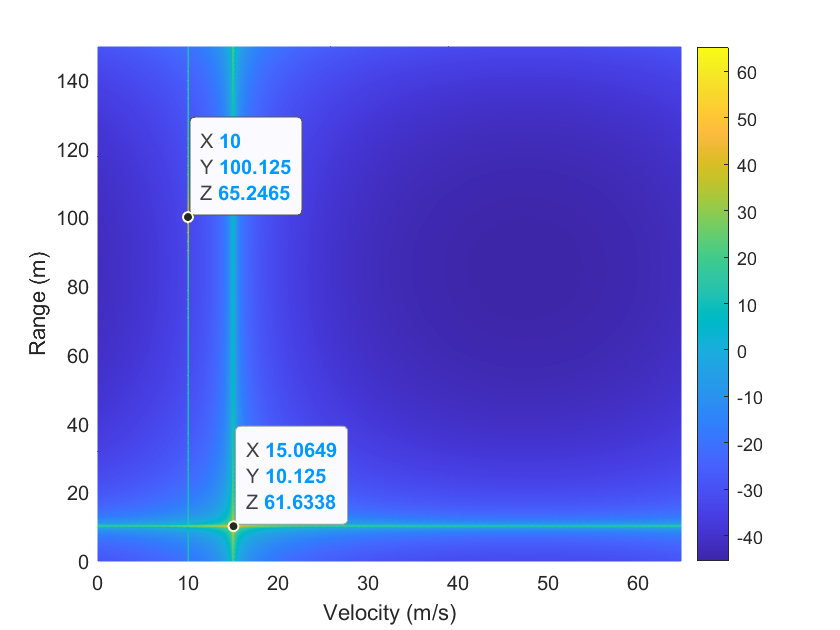
\includegraphics[width=0.4\textwidth]{rdm_range_doppler_compression.png}}}
\caption{RDM Resulting from Range and Doppler Compression.}
\label{rdm_range_doppler_compression}
\end{figure}
\noindent
The measured ranges and velocities are approximately equivalent to the ranges and velocities of the targets. Note that the measured range will be influenced by the doppler shift and measurement resolution of the Fast-Time FFT. The doppler (or velocity) axis will be influenced by the measurement resolution of the Slow-Time FFT.
\noindent
The received power from each target return is related to the target range and RCS by the following equation:
\begin{equation}
P_r \propto \frac{\sigma}{R^4}
\end{equation}
Using the range and RCS of each target, the predicted return power is the same. However, the return of the second target is slightly larger than the return of the first target. This occurs because the first target return has a greater straddle loss. 
\section{Amplitude Compensation}
\label{amp_comp_section}
The targets in Fig. \ref{rdm_range_doppler_compression} may be falsely interpreted as having the same RCS. Amplitude compensation ensures that the power of each target return is influenced only by the RCS. Amplitude compensation is performed by scaling each of the reordered fast-time FFT samples by $R^2$, where $R$ is the range corresponding to each range bin.
\begin{figure}[H]
\centerline{\fbox{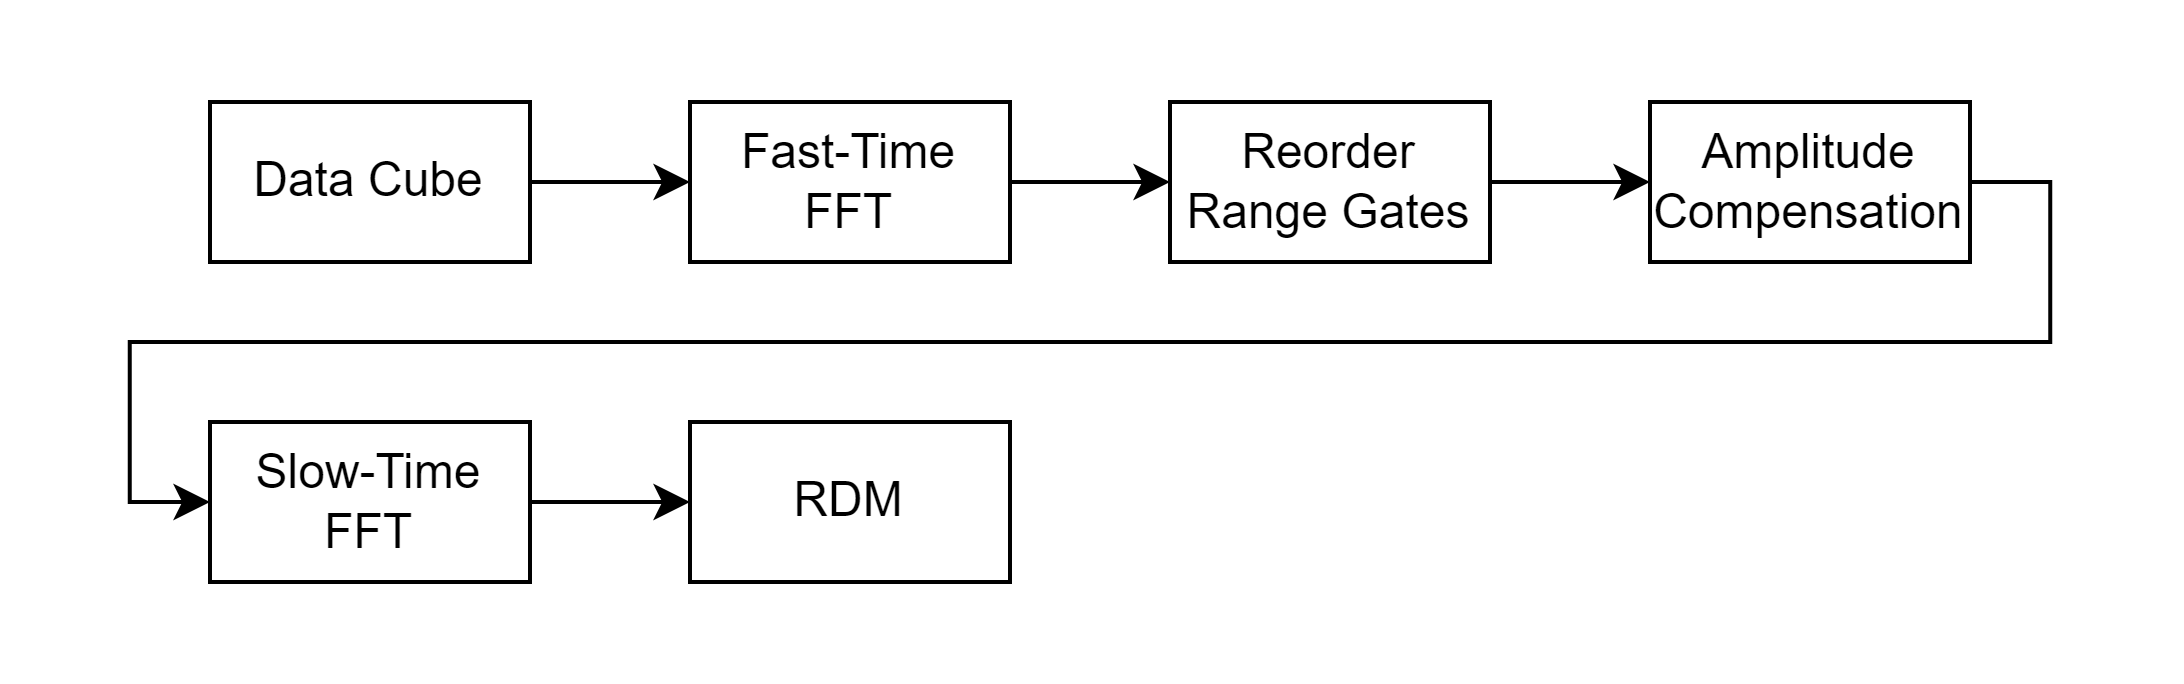
\includegraphics[width=0.4\textwidth]{amplitude_compensation_bd.png}}}
\caption{RDM Generation with Amplitude Compensation.}
\end{figure}
Consider two targets returns that are received in the presence of thermal noise with a power of $0.0001W$. Let the range of both targets be $10m$. Let the velocity of the first target be $15m/s$ and the velocity of the second target be $14m/s$. Finally, let the RCS of the first target be $100m^2$ and the RCS of the second target be $1m^2$. Then, the RDM with amplitude compensation is shown in Fig. \ref{rdm_amplitude_compensation}.
\begin{figure}[H]
\centerline{\fbox{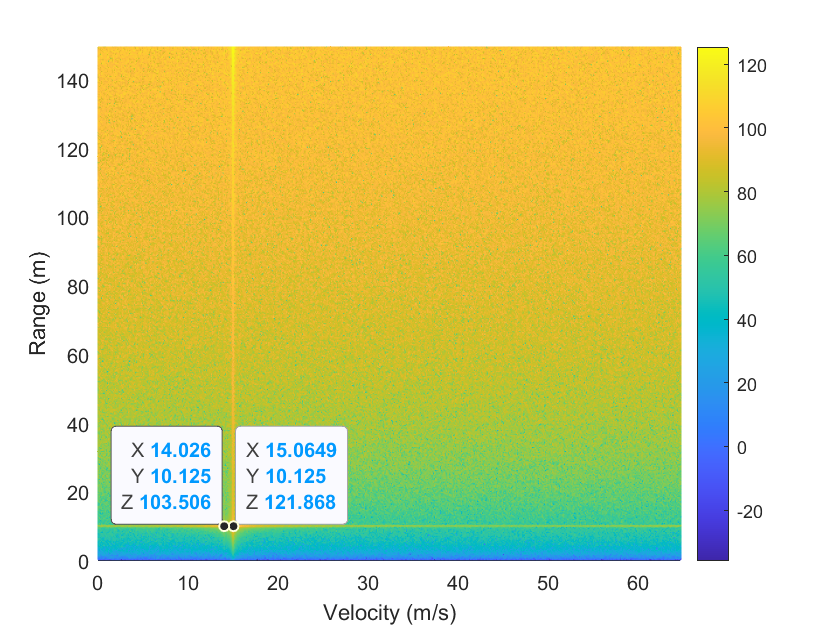
\includegraphics[width=0.4\textwidth]{rdm_amplitude_compensation.png}}}
\caption{RDM after Amplitude Compensation.}
\label{rdm_amplitude_compensation}
\end{figure}
\noindent
Amplitude compensation should ensure that the return of each target is a function of only RCS. Because the RCS of the first target is 20dB greater than that of the second, we expect the first target return to be 20dB greater than the second. This is approximately the case in the RDM. Any discrepancies can be linked to straddle loss.
\section{Range and Doppler Windowing}
In the RDM shown in Fig. \ref{rdm_amplitude_compensation}, the second target return can be difficult to distinguish from the sidelobes of the first target return. This is even more apparent in the closeup shown in Fig. \ref{rdm_amplitude_compensation_close}.
\begin{figure}[H]
\centerline{\fbox{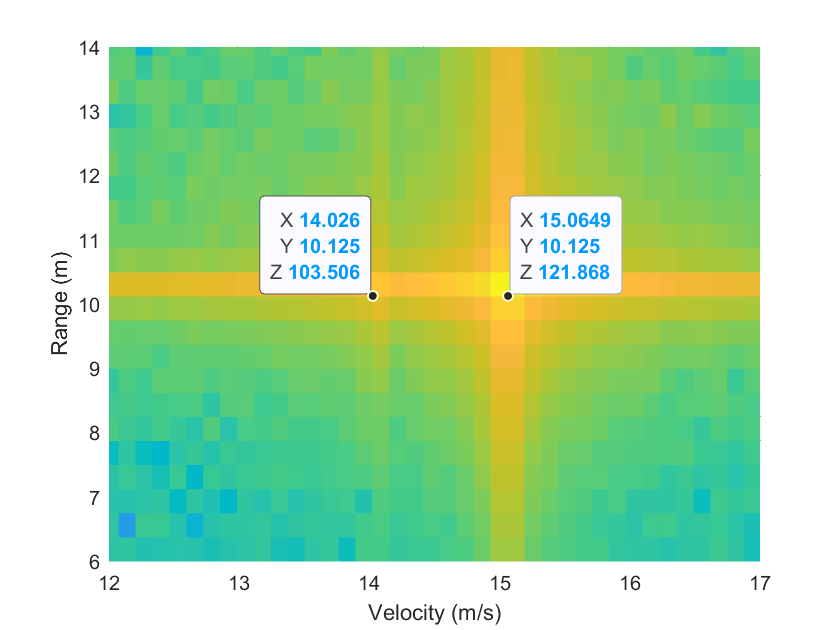
\includegraphics[width=0.4\textwidth]{rdm_amplitude_compensation_close.png}}}
\caption{Closeup of Target Returns.}
\label{rdm_amplitude_compensation_close}
\end{figure}
\noindent
Windowing the input to the fast-time and slow-time FFT can reduce the sidelobe levels and make the two targets more distinguishable. The signal processing chain with the added FFT windows is shown in Fig. \ref{fft_windowing_bd}.
\begin{figure}[H]
\centerline{\fbox{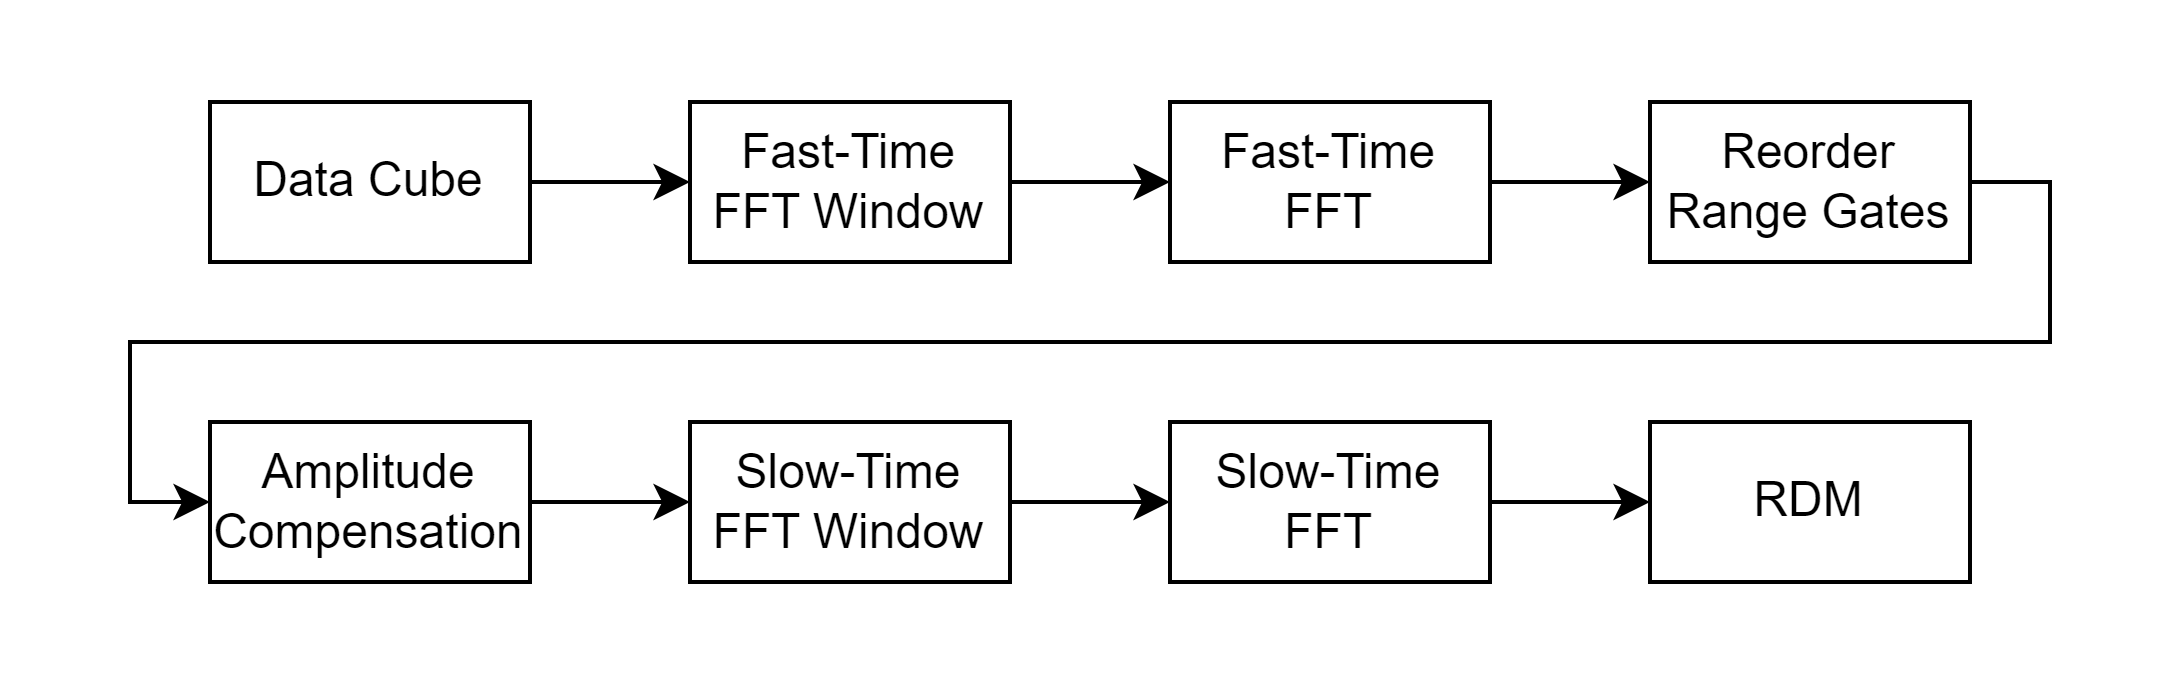
\includegraphics[width=0.4\textwidth]{fft_windowing_bd.png}}}
\caption{Full Signal Processing Chain with Windowing.}
\label{fft_windowing_bd}
\end{figure}
If the targets described in Section \ref{amp_comp_section} are processed using fast-time and slow-time hamming windows,
% before the fast-time and slow-time FFT, the 
%If hamming windows are used in the fast-time and slow-time FFT, the resulting RDM 
%If the targets used to generate Fig. \ref{RDM1} are passed through a radar system with hamming windowing, 
the resulting RDM will be given by Fig. \ref{rdm_fft_windowing}.
\begin{figure}[H]
\centerline{\fbox{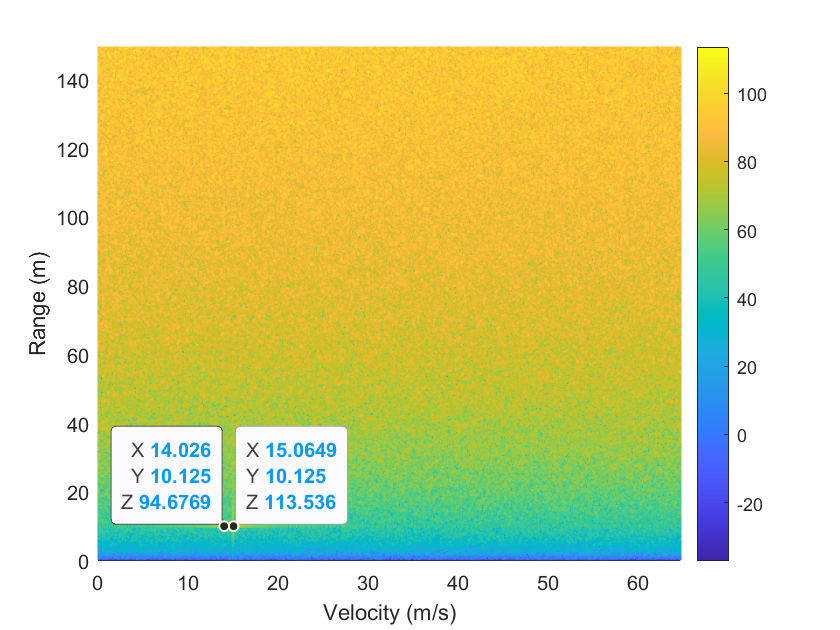
\includegraphics[width=0.4\textwidth]{rdm_fft_windowing.png}}}
\caption{RDM with Added Range and Doppler Windows.}
\label{rdm_fft_windowing}
\end{figure}
\noindent
The range and doppler windows increase the mainlobe width and decrease the magnitude of the range and doppler FFTs. This leads to reduced RDM peaks. The sidelobes in Fig. \ref{rdm_fft_windowing} are significantly lower than the sidelobes of Fig. \ref{rdm_amplitude_compensation}. The reduced sidelobes are even more apparent after zooming on the target returns.
\begin{figure}[H]
\centerline{\fbox{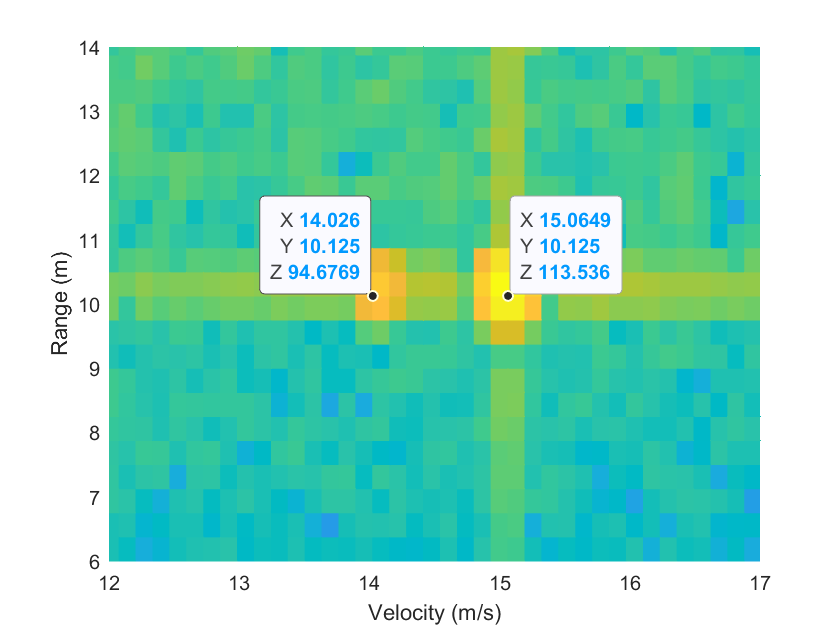
\includegraphics[width=0.4\textwidth]{rdm_fft_windowing_close.png}}}
\caption{Closeup of Target Returns.}
\label{rdm_fft_windowing_close}
\end{figure}
\section{Measurement Limitations}
The range and velocity measurements from the RDM are limited by the range resolution, doppler resolution, range ambiguity, and doppler ambiguity of the system. The range resolution of the system is given by the following equation:
\begin{equation}
\Delta R = \frac{c}{2\beta} = 0.375m
\end{equation}
The doppler resolution of the system is given by the following equation:
\begin{equation}
\Delta F_d = \frac{PRF}{M} = \frac{1}{M\cdot PRI} \approx 66.67Hz
\end{equation}
This corresponds to the following velocity resolution :
\begin{equation}
\Delta v = \frac{\Delta F_d \cdot \lambda}{2} = \frac{\Delta F_d \cdot c}{2f_c} \approx 0.1299 m/s
\end{equation}
The range ambiguity of a conventional radar system is the radar corresponding to a PRI. 
\begin{equation}
R_{ua} = \frac{c \cdot PRI}{2} 
\end{equation}
Because the given radar system leverages stretch processing, some of the unambiguous range is sacrificed for a lower sampling rate. The unambiguous range of the given radar system is described as follows:
\begin{equation}
\label{Rw CPI0}
R_w = \frac{c T_w}{2} = \frac{c F_s \tau}{2\beta} = 150m
\end{equation}
The unambiguous doppler shift of the system is given by the following equation:
\begin{equation}
F_{ua} = PRF = \frac{1}{PRI} = 50kHz
\end{equation}
This results in the following unambiguous velocity:
\begin{equation}
\label{vua CPI0}
v_{ua} = \frac{PRF\cdot\lambda}{2} = \frac{\lambda}{2\cdot PRI} \approx 64.9351m/s 
\end{equation}
If a target is at a range of $200m$ and a velocity of $80m/s$, the target will alias in both velocity in range. If the unambiguous velocity interval is defined as $[0, v_{ua})$, the apparent velocity will be
\begin{equation}
v_a = v - nv_{ua} = 80 - 1 \cdot 64.9351 \approx 15.0649m/s
\end{equation}
and the apparent range will be
\begin{equation}
R_a = R - nR_{ua} = 200 - 150 = 50m
\end{equation}
If the RCS of the target return is $10000 m^2$ and the thermal noise power is $10^{-8}W$, the resulting RDM will be given by
Fig. \ref{rdm_ambiguous_target}.
\begin{figure}[H]
\centerline{\fbox{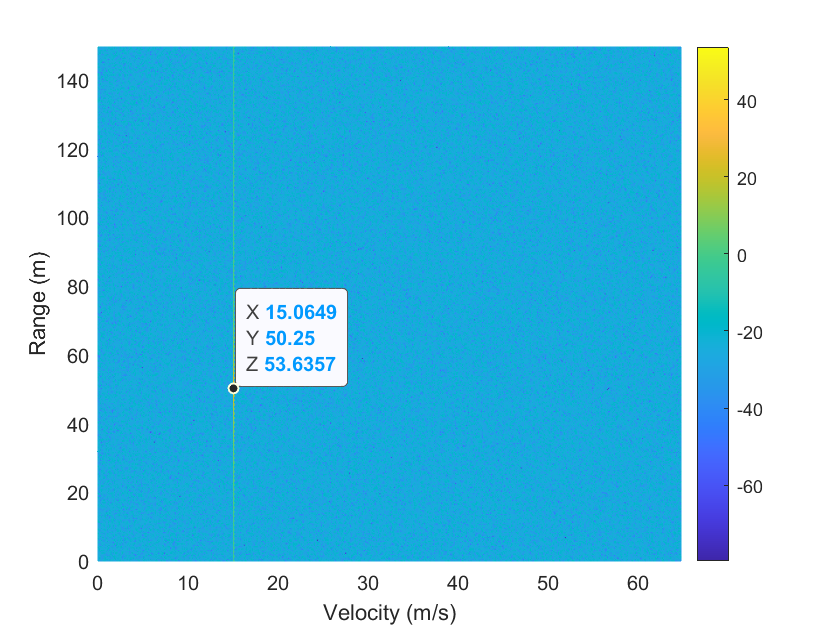
\includegraphics[width=0.4\textwidth]{rdm_ambiguous_target.png}}}
\caption{RDM with Target Placed in Ambiguous Location.}
\label{rdm_ambiguous_target}
\end{figure}
\noindent
Note that the measured range is not exactly $50m$ due to range-doppler coupling and the range resolution of the system.
\par
To correctly detect the target's range and velocity, the system's unambiguous range and velocity must be increased. The unambiguous velocity is inversely proportional to the PRI. Therefore, to increase the unambiguous velocity, the PRI must be reduced. If the PRI is reduced to $20\mu s$, the unambiguous velocity will be given by the following:
\begin{equation}
v_{ua} = \frac{\lambda}{2\cdot PRI} \approx 97.4026 m/s
\end{equation}
Note that the PRI is limited by the pulse length $\tau$ and the time it takes the VCO to stabilize between chirps. If the time between chirps is held constant, the pulse length will need to be reduced to $10\mu s$. Depending on the performance of the VCO, the chirp bandwidth may also need to be reduced. In this document, the VCO is assumed to be tolerant of the increased chirp rate. This ensures that the existing range resolution is preserved.
\par
To increase the system's unambiguous range, the sample rate of the ADC must be increased. To provide an unambiguous range of 300m with the reduced pulse length, the ADC sample rate must be increased to:
\begin{equation}
F_s = \frac{2\beta R_w}{c\tau} = 80MHz 
\end{equation}
Using the reduced PRI and increased sample rate, the target at a range of $200m$ and a velocity of $80m/s$ can be resolved without ambiguity. This is illustrated in Fig. \ref{rdm_unambiguous_target}.
\begin{figure}[H]
\centerline{\fbox{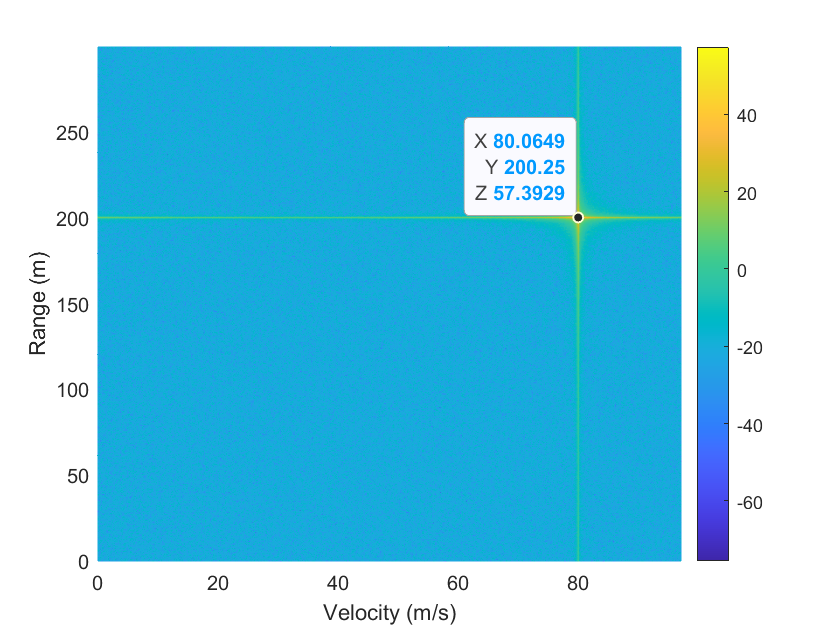
\includegraphics[width=0.4\textwidth]{rdm_unambiguous_target.png}}}
\caption{RDM with Target Placed in Unambiguous Location.}
\label{rdm_unambiguous_target}
\end{figure}
If the sample rate of the ADC cannot be increased, another solution involves using two CPIs with unique sample rates and PRIs. One possible set of CPI configurations uses the parameters given in Table \ref{Parameter Table} for the first CPI and adjusts the sample rate and PRI of the second CPI to $15MHz$ and $40\mu s$ respectively. The unambiguous range and velocity for the first CPI are given by equations \ref{Rw CPI0} and \ref{vua CPI0} respectively. The unambiguous range and velocity for the second CPI are given as follows:
\begin{equation}
R_w = \frac{c F_s \tau}{2\beta} = 112.5m
\end{equation}
\begin{equation}
v_{ua} = \frac{\lambda}{2\cdot PRI} \approx 48.7013 m/s
\end{equation}
The unambiguous range of the system can be expressed in terms of each CPI's unambiguous range as follows:
\begin{equation}
\label{Rua}
R_{uas} = \text{lcm}(R_{ua0}, R_{ua1}) = 450m
\end{equation}
The unambiguous velocity of the system can be expressed in a form similar to equation \ref{Rua}. However, due to rounding errors in the unambiguous velocities, it is preferable to first solve for the base interval $T_g$ and set of staggers $\{k_p\}$. The base interval and set of staggers are given by the following equations:
\begin{equation}
T_g = \text{gcd}(PRI_0,PRI_1) = 10\mu s
\end{equation}
\begin{equation}
k_0 = 3 \quad k_1 = 4
\end{equation}
Using the base interval and set of staggers, the system's unambiguous doppler shift can be expressed as follows:
\begin{equation}
F_{bs} = \frac{1}{T_g}\text{lcm}\left(\frac{1}{k_0},\frac{1}{k_1}\right) = 100kHz
\end{equation}
Finally, the system's unambiguous velocity can be computed as follows:
\begin{equation}
v_{uas} = \frac{F_{bs}\lambda}{2} \approx 194.805m/s
\end{equation}
The RDM for the first CPI is shown in Fig. \ref{rdm_ambiguous_target}, and the RDM for the second CPI is shown in Fig. \ref{multiple_cpi_rdm}.
\begin{figure}[H]
\centerline{\fbox{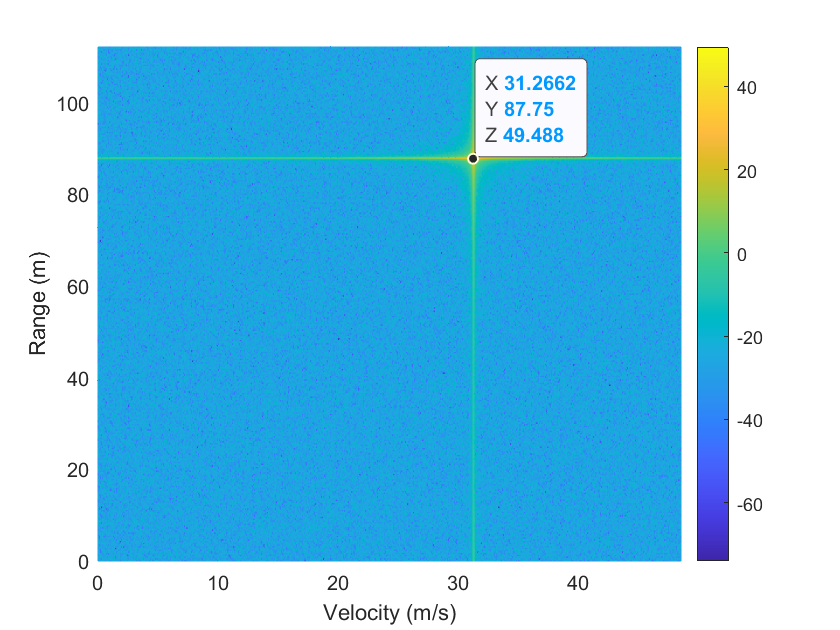
\includegraphics[width=0.4\textwidth]{multiple_cpi_rdm.png}}}
\caption{RDM for Second CPI in Multiple CPI System.}
\label{multiple_cpi_rdm}
\end{figure}
\noindent
The velocity and range of the target can be computed by examining the set of ranges and velocities that may have lead to the measurements in each CPI. For the first CPI's RDM, illustrated in Fig. \ref{rdm_ambiguous_target}, possible target ranges are given below:
\begin{table}[H]
\caption{Possible Target Ranges Derived from First CPI}
\label{Range CPI0}
\begin{tabularx}{0.5\textwidth}{| X | X |}
\hline
Ambiguity Interval & Range \\
\hline
0 & 50.25m \\
\hline
1 & 200.25m \\
\hline
2 & 350.25m \\
\hline
\end{tabularx}
\end{table}
\noindent
For the second CPI's RDM, illustrated in Fig. \ref{multiple_cpi_rdm}, possible target ranges are given below:
\begin{table}[H]
\caption{Possible Target Ranges Derived from Second CPI}
\label{Range CPI1}
\begin{tabularx}{0.5\textwidth}{| X | X |}
\hline
Ambiguity Interval & Range \\
\hline
0 & 87.75m \\
\hline
1 & 200.25m \\
\hline
2 & 312.75m \\
\hline
3 & 425.25m \\
\hline
\end{tabularx}
\end{table}
\noindent
The true range of the target is the closest pair of measurements, which is 200.25m. Note that this matches the result shown in Fig. \ref{rdm_unambiguous_target}. The velocity of the target can be found in a similar manner. For the first CPI's RDM, illustrated in Fig. \ref{rdm_ambiguous_target}, possible target velocities are given below:
\begin{table}[H]
\caption{Possible Target Velocities Derived from First CPI}
\label{Velocity CPI0}
\begin{tabularx}{0.5\textwidth}{| X | X |}
\hline
Ambiguity Interval & Velocity \\
\hline
0 & 15.0649m/s \\
\hline
1 & 80m/s \\
\hline
2 & 144.9351m/s \\
\hline
\end{tabularx}
\end{table}
\noindent
For the second CPI's RDM, illustrated in Fig. \ref{multiple_cpi_rdm}, possible target velocities are given below:
\begin{table}[H]
\caption{Possible Target Velocities Derived from Second CPI}
\label{Velocity CPI1}
\begin{tabularx}{0.5\textwidth}{| X | X |}
\hline
Ambiguity Interval & Velocity \\
\hline
0 & 31.2662m/s \\
\hline
1 & 79.9675m/s \\
\hline
2 & 128.6688m/s \\
\hline
3 & 177.3701m/s \\
\hline
\end{tabularx}
\end{table}
\noindent
The true velocity of the target is the closest pair of measurements, which is approximately 80m/s. Note that this result approximately matches the result shown in Fig. \ref{rdm_unambiguous_target}. Any measurement discrepancies occur due different velocity resolutions in each of the CPIs.
\section{Conclusion}
In this document, an LFM radar system leveraging stretch processing was examined. The stretch processing receiver performed additional analog processing before the ADC to reduce the sample rate of the system. The sampled ADC signal was then shaped in data cube. MATLAB was used to generate received data cubes for different scenarios and then process them. The result of this operation was a set of range doppler matrices (RDMs). Key processing steps included range and doppler compression, which provided range and velocity estimates for each target. Other processing steps included amplitude compensation, which ensured each target's return power depended only on the RCS, and FFT windowing, which reduced sidelobe levels. Finally, the measurement limitations of the system were discussed (range resolution, doppler resolution, range ambiguity, and doppler ambiguity). Two methods for extending the ambiguities were also provided. The first method involved reducing the PRI and pulse length, while increasing the sampling rate. The second method involved using two CPIs with slightly different PRIs and sampling rates. Both methods were proven to extend the system's ambiguities. The concepts discussed in this document are crucial for the design and implementation of an LFM radar system leveraging stretch processing. However, they can also be applied to many other radar systems.
\onecolumn
\pagebreak
\appendices
\section{MATLAB Source Code}
\label{matlab_code}
\lstset{style=Matlab-editor}
\lstinputlisting{Project2_Sowatzke.m}
\raggedbottom
\pagebreak
\lstinputlisting{radar.m}
\raggedbottom
\end{document}
